% https://tex.stackexchange.com/a/240917/173708
\documentclass[tikz,border=10pt]{standalone}
\usepackage{tikz}

\usetikzlibrary{arrows,calc,decorations.pathmorphing,positioning,decorations.markings}

\tikzset{
    % build the shaded rectangle
    shadedrec/.style={
        rectangle,
        draw=black,
        top color=gray,        % this is part of the shade
        bottom color=white,    % this is part of the shade
        shading angle={135},   % this is part of the shade
        text width=3cm,
        inner sep=1em,
        rounded corners=1.2ex,
        very thick,
        text centered},
    snake arrow/.style={
        decorate,
        decoration={zigzag,amplitude=3mm,segment length=5mm,post length=0mm}},
    damper/.style={
        very thick,
        decoration={markings,  
        mark connection node=dmp,
        mark=at position 0.5 with 
        {
            \node (dmp) [very thick,transform shape,text width=.3cm,rotate=-90,minimum height=3pt,draw=none, fill=black,outer xsep=2pt, outer ysep=1pt] {};
            \draw [very thick] ($(dmp.north east)+(-.6pt,0)$) -- ($(dmp.south east)+(-.6pt,0)$) -- ($(dmp.south west)+(-.6pt,0)$) -- ($(dmp.north west)+(-.6pt,0)$);
            \draw [very thick,rotate=-90] ($(dmp.north)+(0,-5pt)$) -- ($(dmp.north)+(0,5pt)$);
        }
    }, decorate}
}

\begin{document}
\pagestyle{empty}

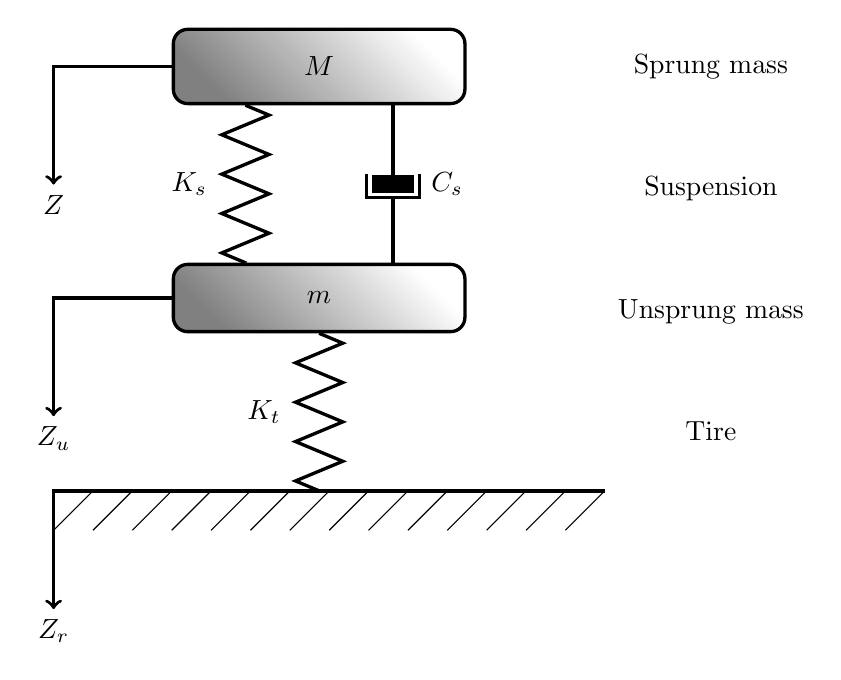
\begin{tikzpicture}
    % Shapes
    \node[shadedrec, anchor=center] (S1) at (4,3) {$M$};
    \node[shadedrec, anchor=center, below=2 of S1] (S2) {$m$};

    %Nodes side
    \node[anchor=center,text centered,right=2cm of S1.east] (sm) {Sprung mass};
    \node[below=of sm] (susp) {Suspension};
    \node[below=of susp] (usm) {Unsprung mass};
    \node[below=of usm] {Tire};

    % Paths

    %side arrows
    \draw[->,very thick] (S1.west) -- ++ (-1.5,0) -- ++ (0,-1.5) node[below] {$Z$};
    \draw[->,very thick] (S2.west) -- ++ (-1.5,0) -- ++ (0,-1.5) node[below] {$Z_u$};

    %zigzag lines
    \draw[very thick, snake arrow] ($(S1.south west)!.5!(S1.south)$) -- ++ (0,-2) node[left,midway,xshift=-1em] {$K_s$};
    \draw[very thick, snake arrow] (S2.south) -- ++ (0,-2) 
        node[left,midway,xshift=-1em] {$K_t$};

    %Connector shape
    \draw[damper] ($(S2.north east)!.5!(S2.north)$) -- ($(S1.south east)!.5!(S1.south)$) node[right,midway,xshift=1em] {$C_s$};

    % Road
    \coordinate (A) at ($(S2.west)+(5.5,-2.45)$);
    \draw[->,very thick] (A) -- ++(-7,0) -- ++ (0,-1.5) node[below] {$Z_r$};

    \begin{scope}[shift={($(S2.west)+(-1.5,-2.45)$)}]
        \foreach \x in {0.5,1,...,7} { %This one draws the little diagonal lines
        \draw (\x,0) -- ({\x-.5},-.5);
        }
    \end{scope} 
\end{tikzpicture}

\end{document}